\documentclass[]{article}

\usepackage[margin=1.0in]{geometry}
\usepackage{graphicx}
\usepackage{float}
\usepackage{amsmath}
\usepackage{amssymb}
\usepackage{hyperref}
\usepackage{array}

\pagestyle{plain}

\begin{document}
%\begin{minipage}{6in}
%\centering
%\raisebox{-0.5\height}{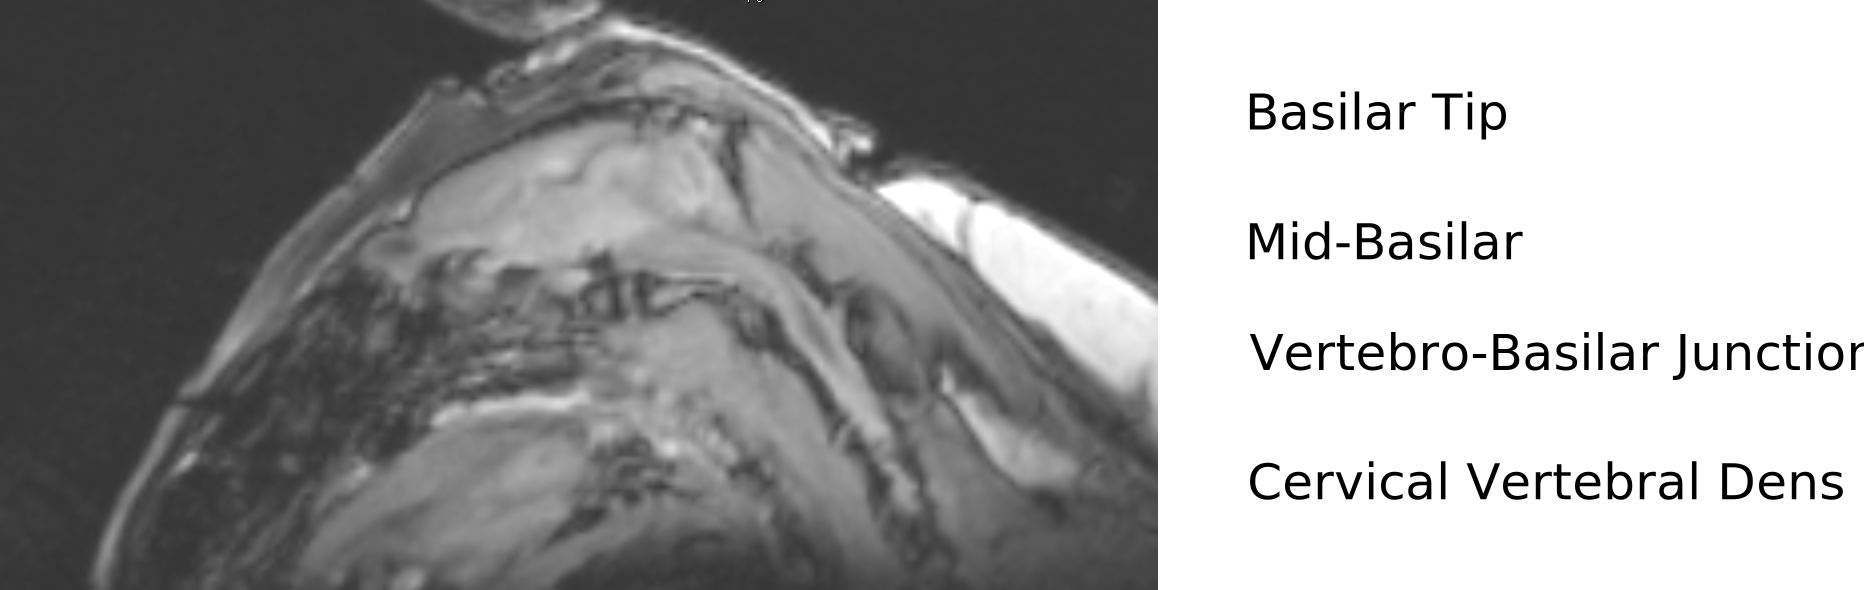
\includegraphics[height=0.75in]{brain.pdf}}
%\hspace*{.2in}
%\raisebox{-0.5\height}{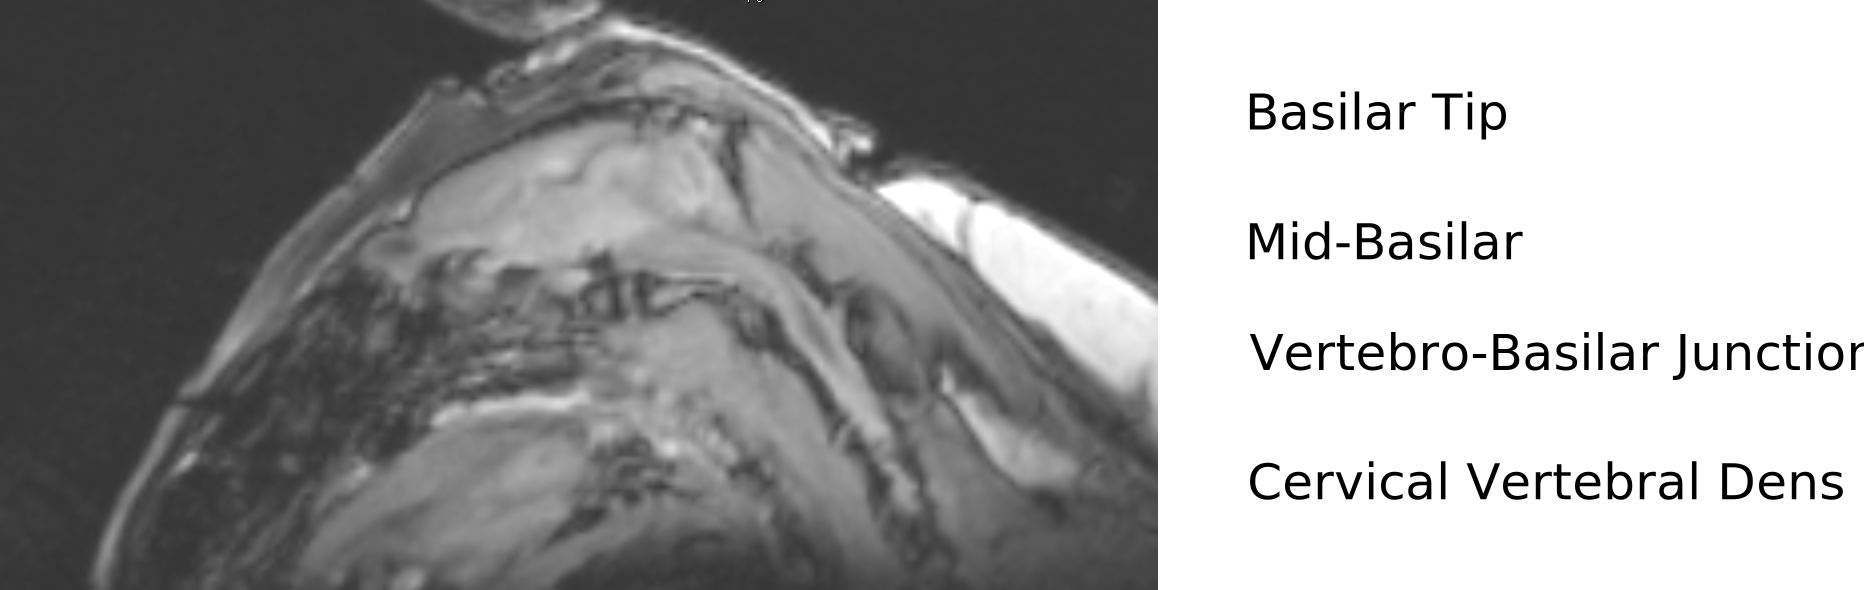
\includegraphics[height=0.3in]{brain.pdf}}
%\end{minipage}

\begin{figure}[H]
\begin{center}
\raisebox{-0.5\height}{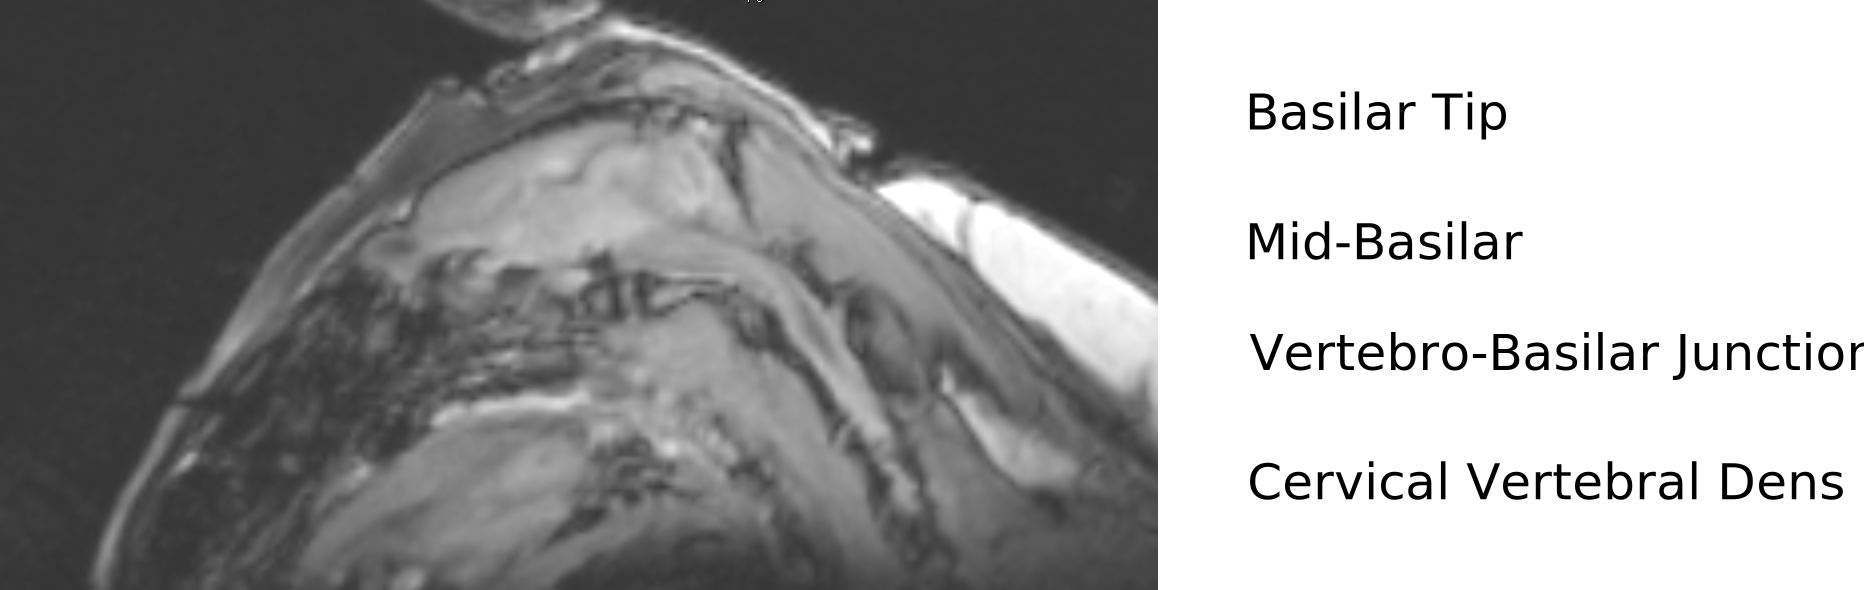
\includegraphics[scale=0.8]{brain.pdf}}
\hspace{0.2cm}
\raisebox{-0.5\height}{\includegraphics[scale=1.0]{../config/legend.pdf}} \\
\vspace{0.5cm}
\begin{tabular}{m{5cm}m{20cm}}
VEP, Distal Basilar Artery, recording from guidewire against a Ag/AgCl reference &
\includegraphics[scale=0.250]{../vep/matlab_data/_Fri_11_04_2014_15_25_33_vep_.pdf} \\
VEP, Distal Basilar Artery, recording from guidewire &
\includegraphics[scale=0.250]{../vep/matlab_data/_Fri_11_04_2014_15_33_56_vep_.pdf} \\
VEP Dead Control &
\includegraphics[scale=0.250]{../vep/matlab_data/_Fri_11_04_2014_17_00_46_vep_.pdf} \\
\end{tabular}
\caption{Rabbit 6 VEP.}
\end{center}
\end{figure}

\begin{figure}[H]
\begin{center}
\raisebox{-0.5\height}{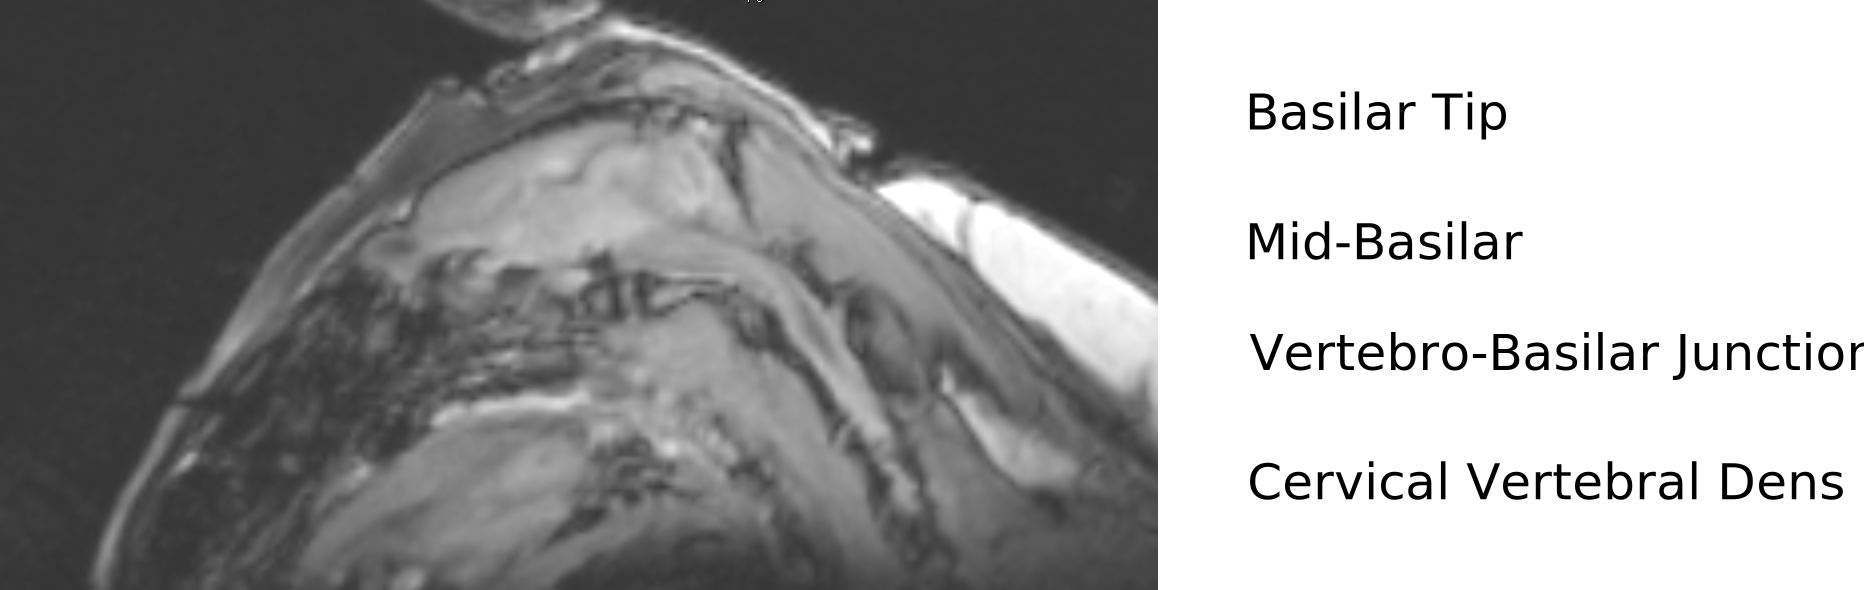
\includegraphics[scale=0.8]{brain.pdf}}
\hspace{0.2cm}
\raisebox{-0.5\height}{\includegraphics[scale=1.0]{../config/legend.pdf}} \\
\vspace{0.5cm}
\begin{tabular}{m{5cm}m{20cm}}
%SSVEP 40 Hz, no signal on anything &
%\includegraphics[scale=0.250]{../ssvep/matlab_data/_Fri_11_04_2014_15_27_09_ssvep_.pdf} \\
SSVEP 40 Hz, distal basilar artery, recording from guidewire &
\includegraphics[scale=0.250]{../ssvep/matlab_data/_Fri_11_04_2014_15_35_24_ssvep_.pdf} \\
SSVEP 12 Hz, distal basilar artery, recording from guidewire &
\includegraphics[scale=0.250]{../ssvep/matlab_data/_Fri_11_04_2014_15_42_09_ssvep_.pdf} \\
SSVEP 12 Hz Dead Control &
\includegraphics[scale=0.250]{../ssvep/matlab_data/_Fri_11_04_2014_17_02_31_ssvep_.pdf} \\
SSVEP 40 Hz Dead Control &
\includegraphics[scale=0.250]{../ssvep/matlab_data/_Fri_11_04_2014_17_03_23_ssvep_.pdf} \\
\end{tabular}
\caption{Rabbit 6 SSVEP.}
\end{center}
\end{figure}

\begin{figure}[H]
\begin{center}
\raisebox{-0.5\height}{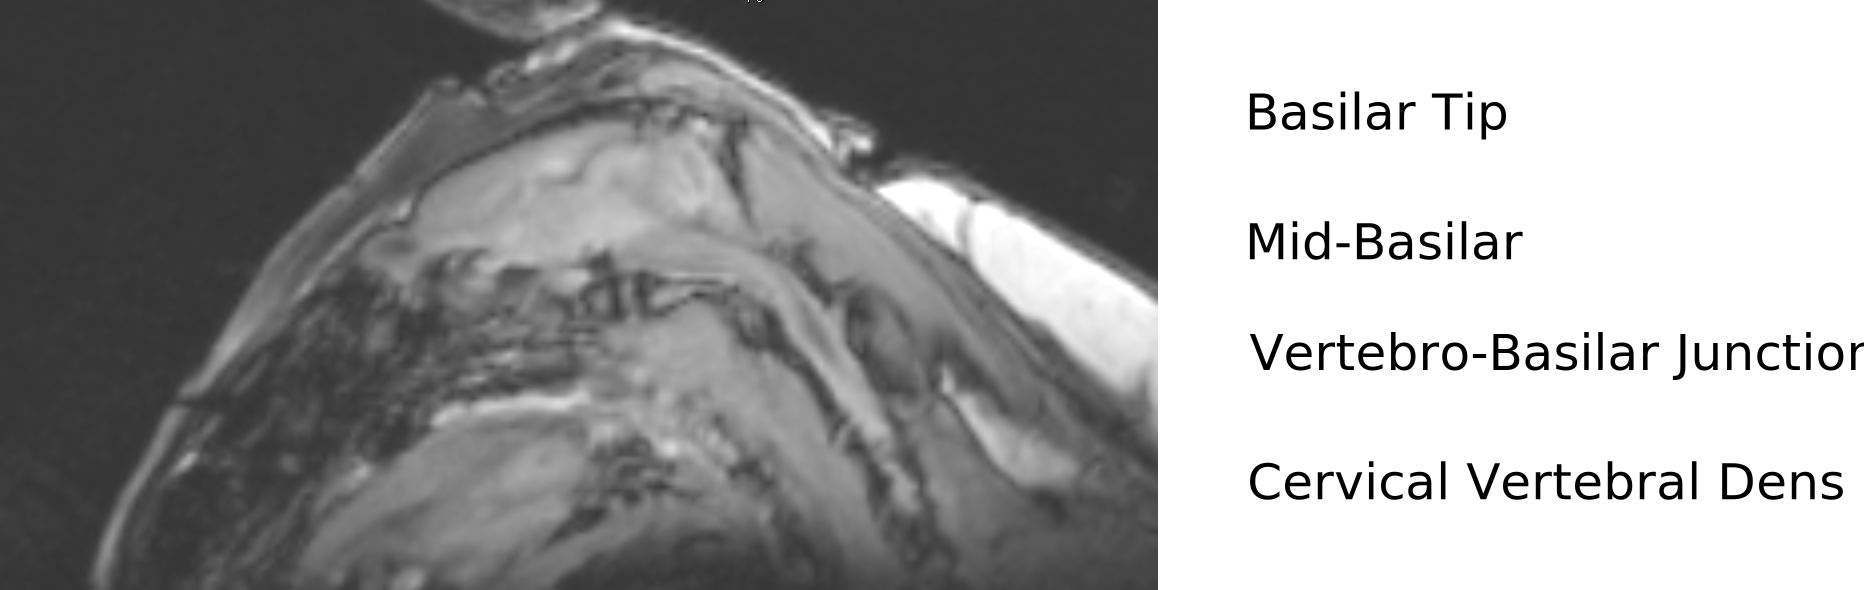
\includegraphics[scale=0.8]{brain.pdf}}
\hspace{0.2cm}
\raisebox{-0.5\height}{\includegraphics[scale=1.0]{../config/legend.pdf}} \\
\vspace{0.5cm}
\begin{tabular}{m{5cm}m{20cm}}
VEP, angled glide catheter (ag/agcl) in abdominal descending aorta &
\includegraphics[scale=0.250]{../vep/matlab_data/_Tue_15_04_2014_15_45_35_vep_.pdf} \\
SSVEP 40 Hz, angled glide catheter (ag/agcl) in abdominal descending aorta &
\includegraphics[scale=0.250]{../ssvep/matlab_data/_Tue_15_04_2014_15_48_37_ssvep_40_.pdf} \\
SSVEP 12 Hz, angled glide catheter (ag/agcl) in abdominal descending aorta &
\includegraphics[scale=0.250]{../ssvep/matlab_data/_Tue_15_04_2014_15_49_46_ssvep_12.pdf}
\end{tabular}
\caption{Rabbit 7.}
\end{center}
\end{figure}

\begin{figure}[H]
\begin{center}
%\raisebox{-0.5\height}{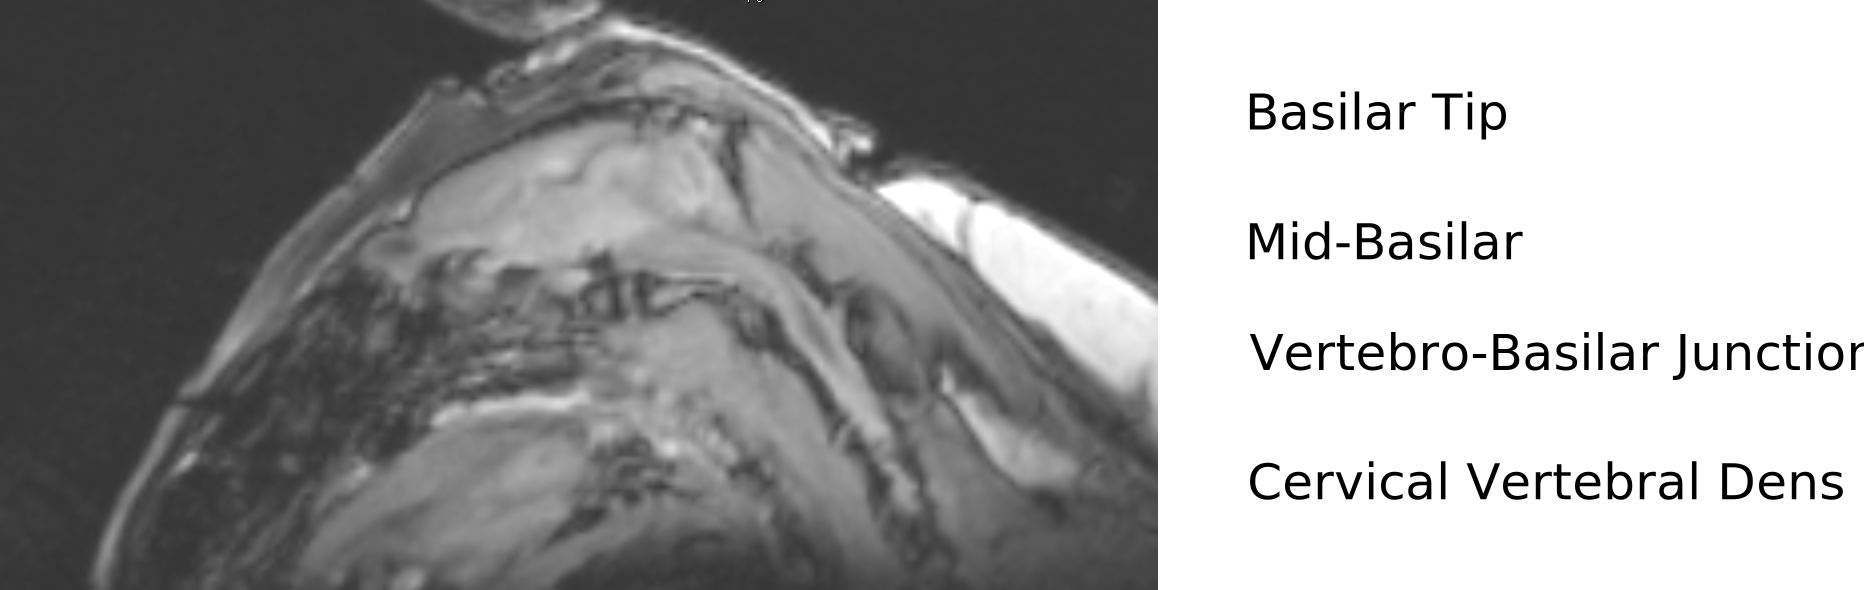
\includegraphics[scale=0.8]{brain.pdf}}
%\hspace{0.2cm}
%\raisebox{-0.5\height}{\includegraphics[scale=1.0]{../config/legend.pdf}} \\
%\vspace{0.5cm}
\begin{tabular}{m{5cm}m{20cm}}
VEP, Baseline Brain Recordings - no catheter in the rabbit - endo not hooked up &
\includegraphics[scale=0.150]{../vep/matlab_data/_Thu_24_04_2014_10_24_11_vep_.pdf} \\
VEP right eye, X-pedion wire through echelon-10, basilar tip (via left vert); wire projects slightly beyond the catheter (documented on imaging) &
\includegraphics[scale=0.150]{../vep/matlab_data/_Thu_24_04_2014_12_55_56_vep_.pdf} \\
12:55:56 - VEP right eye, 3 minutes, GND: nose -X-pedion wire through echelon-10, basilar tip (via left vert); wire projects slightly beyond the catheter (documented on imaging) &
\includegraphics[scale=0.150]{../vep/matlab_data/_Thu_24_04_2014_12_55_56_vep_.pdf} \\
13:13:22 - VEP  right eye - 3 min -echelon-10, basilar tip (via left vert), Ag/AgCl electrode &
\includegraphics[scale=0.150]{../vep/matlab_data/_Thu_24_04_2014_13_13_22_vep_.pdf} \\
13:31:48 - VEP right eye - 5 min -echelon-10, basilar tip (via left vert), Ag/AgCl electrode &
\includegraphics[scale=0.150]{../vep/matlab_data/_Thu_24_04_2014_13_31_48_vep_5min.pdf} \\
13:47:15 - VEP right eye - 3 minutes- X-pedion wire through echelon-10, wire is just at hub of catheter; catheter remains at basilar tip &
\includegraphics[scale=0.150]{../vep/matlab_data/_Thu_24_04_2014_13_47_15_vep_.pdf} \\
\end{tabular}
\caption{Rabbit 8 VEP.}
\end{center}
\end{figure}

\begin{figure}[H]
\begin{center}
%\raisebox{-0.5\height}{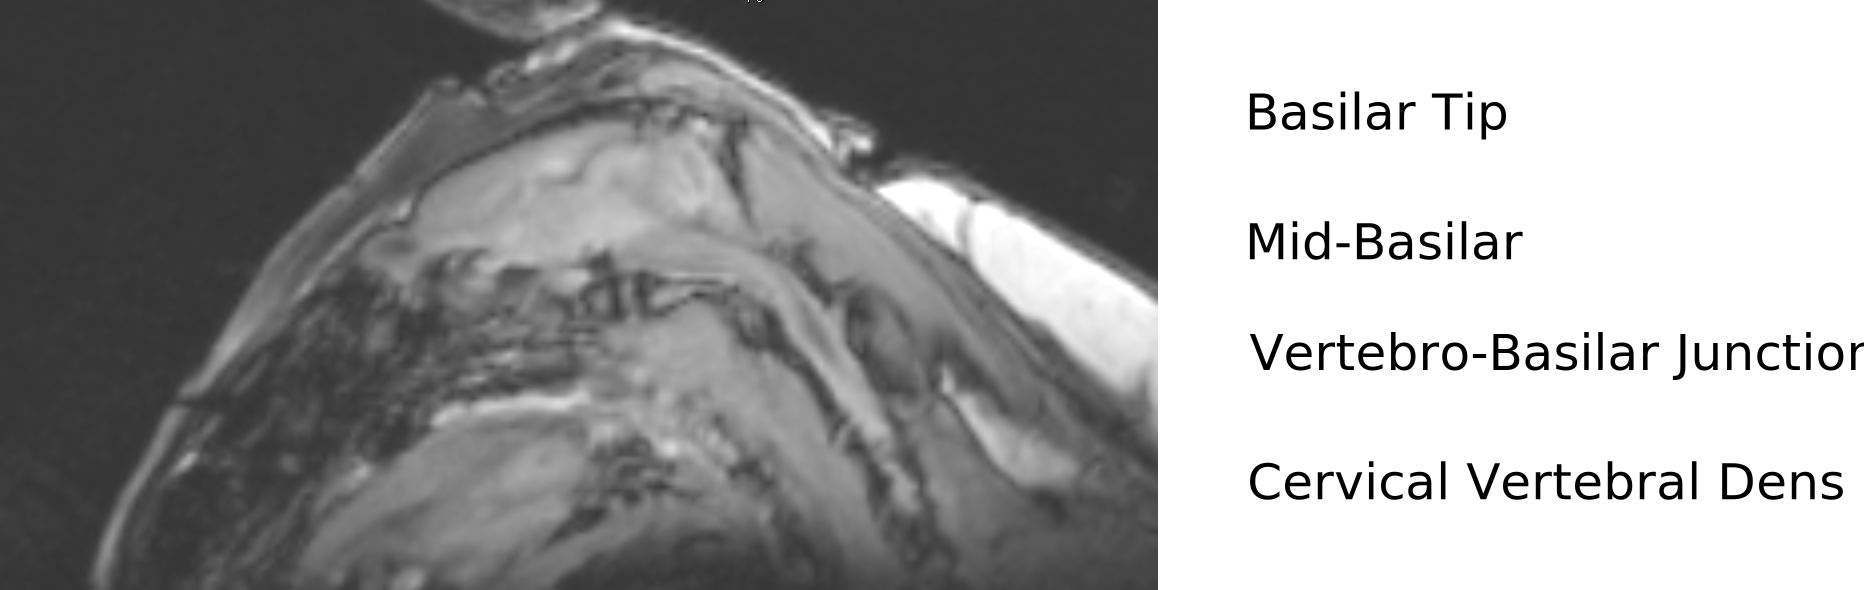
\includegraphics[scale=0.8]{brain.pdf}}
%\hspace{0.2cm}
%\raisebox{-0.5\height}{\includegraphics[scale=1.0]{../config/legend.pdf}} \\
%\vspace{0.5cm}
\begin{tabular}{m{5cm}m{20cm}}
14:03:52 - VEP, 3 min GND: Nose- X-pedion wire, 100 cm (half-length), through echelon 10. Specifically: wire is 100 cm into the catheter (total length of wire is 200cm; hub of sidearm reaches 100cm from proximal end of wire) &
\includegraphics[scale=0.150]{../vep/matlab_data/_Thu_24_04_2014_14_03_52_vep_.pdf} \\
14:20:45 - VEP, 3 min, GND: Nose -X-pedion wire, hub of sidearm reaches 47.3 cm from proximal end of wire (calculated so that wire is 10 cm from catheter tip (assuming 162.7 cm total catheter length: 150cm catheter shaft plus hub material that we measured by hand, plus the length of the sidearm) &
\includegraphics[scale=0.150]{../vep/matlab_data/_Thu_24_04_2014_14_20_45_vep_3min.pdf} \\
14:43:08 - VEP, 3, min - lights in room are ON - X-pedion wire, repositioned just beyond tip of Echelon catheter at tip of basilar, confirmed with imaging; ALL ELECTRONICS ON, 4 PERSONNEL MOVING AND TALKING IN ROOM &
\includegraphics[scale=0.150]{../vep/matlab_data/_Thu_24_04_2014_14_43_08_vep_.pdf} \\
14:46:54 - VEP, 3, min - lights in room are OFF - X-pedion wire, repositioned just beyond tip of Echelon catheter at tip of basilar, confirmed with imaging; ALL ELECTRONICS ON, 4 PERSONNEL MOVING AND TALKING IN ROOM &
\includegraphics[scale=0.150]{../vep/matlab_data/_Thu_24_04_2014_14_46_54_vep_.pdf} \\
15:05:50 - VEP, 3 min - ELECTRONICS OFF (unchanged position X-pedion wire, repositioned just beyond tip of Echelon catheter at tip of basilar,) &
\includegraphics[scale=0.150]{../vep/matlab_data/_Thu_24_04_2014_15_05_50_vep_.pdf}
\end{tabular}
\caption{Rabbit 8 VEP (continued).}
\end{center}
\end{figure}

\begin{figure}[H]
\begin{center}
%\raisebox{-0.5\height}{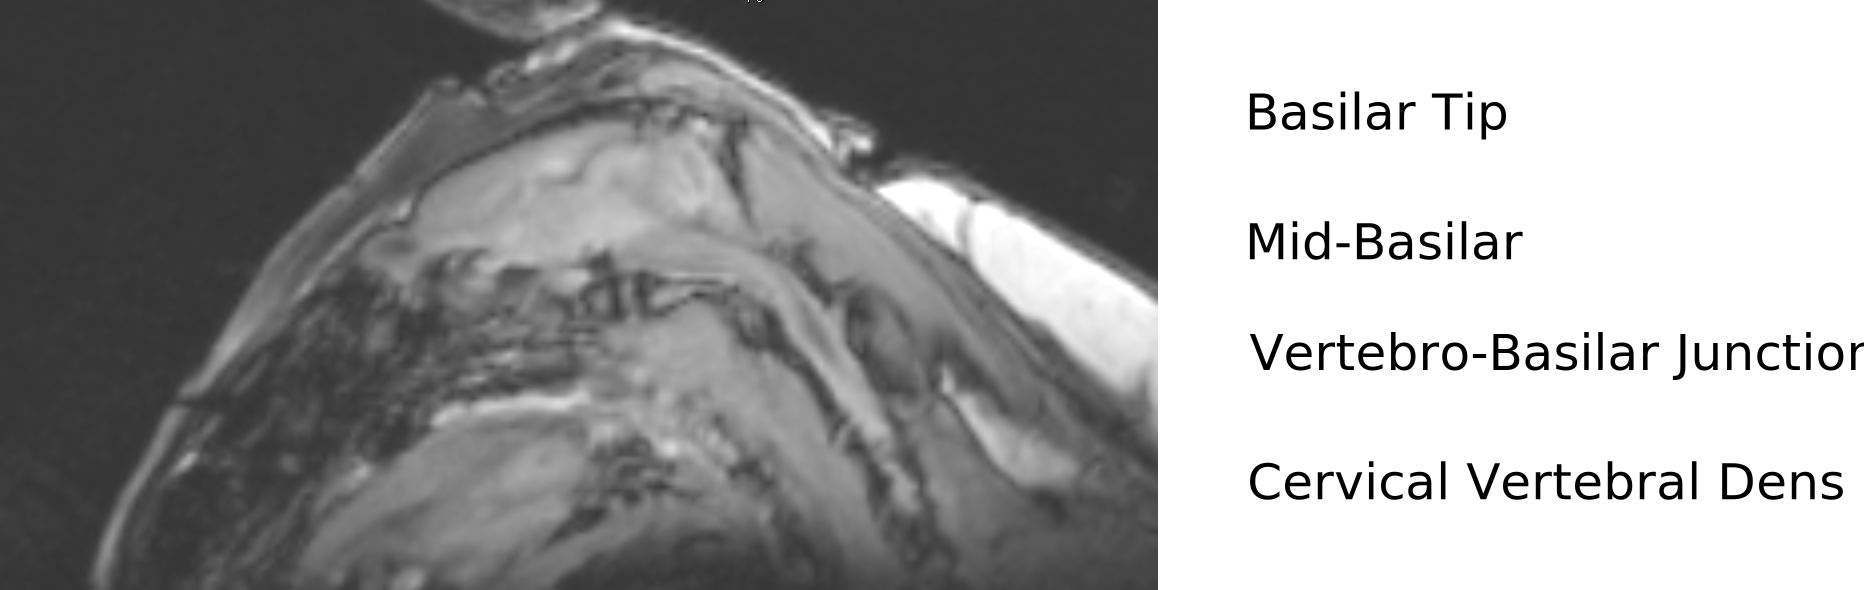
\includegraphics[scale=0.8]{brain.pdf}}
%\hspace{0.2cm}
%\raisebox{-0.5\height}{\includegraphics[scale=1.0]{../config/legend.pdf}} \\
%\vspace{0.5cm}
\begin{tabular}{m{5cm}m{20cm}}
SSVEP, 12 Hz, Baseline Brain Recordings - no catheter in the rabbit - endo not hooked up &
\includegraphics[scale=0.150]{../ssvep/matlab_data/_Thu_24_04_2014_10_36_32_ssvep_.pdf} \\
11:58:44 - SSVEP 12 Hz, GND: Nose - Left Vert - angled glidecath @ osteum of left vert; recording from Ag/AgCl; GND: Nose &
\includegraphics[scale=0.150]{../ssvep/matlab_data/_Thu_24_04_2014_11_58_44_ssvep_.pdf} \\
SSVEP 12 Hz, X-pedion wire through echelon-10, basilar tip (via left vert); wire projects slightly beyond the catheter (documented on imaging) &
\includegraphics[scale=0.150]{../ssvep/matlab_data/_Thu_24_04_2014_13_00_49_ssvep_.pdf} \\
13:23:31 - SSVEP 12 Hz, GND: Nose -echelon-10, basilar tip (via left vert), Ag/AgCl electrode &
\includegraphics[scale=0.150]{../ssvep/matlab_data/_Thu_24_04_2014_13_23_31_ssvep_.pdf} \\
13:52:55 - SSVEP right eye 10 Hz, GND: Nose- X-pedion wire through echelon-10, wire is just at hub of catheter; catheter remains at basilar tip &
\includegraphics[scale=0.150]{../ssvep/matlab_data/_Thu_24_04_2014_13_52_55_ssvep_12hz.pdf} \\
14:07:37 - SSVEP, 12 Hz, GND: Nose- X-pedion wire, 100 cm (half-length), through echelon 10. Specifically: wire is 100 cm into the catheter (total length of wire is 200cm; hub of sidearm reaches 100cm from proximal end of wire) &
\includegraphics[scale=0.150]{../ssvep/matlab_data/_Thu_24_04_2014_14_07_37_ssvep_12hz.pdf} \\
%14:26:57 - SSVEP 12 Hz, GND: Nose -X-pedion wire, hub of sidearm reaches 47.3 cm from proximal end of wire (calculated so that wire is 10 cm from catheter tip (assuming 162.7 cm total catheter length: 150cm catheter shaft plus hub material that we measured by hand, plus the length of the sidearm) &
%14:50:43 - SSVEP - 12 Hz, GND: Nose  - lights in room are OFF - X-pedion wire, repositioned just beyond tip of Echelon catheter at tip of basilar, confirmed with imaging; ALL ELECTRONICS ON, 4 PERSONNEL MOVING AND TALKING IN ROOM &
15:12:45 - SSVEP, 12 Hz - ELECTRONICS OFF (unchanged position X-pedion wire, repositioned just beyond tip of Echelon catheter at tip of basilar,) &
\includegraphics[scale=0.150]{../ssvep/matlab_data/_Thu_24_04_2014_15_12_45_ssvep_12.pdf} \\
15:50:45 - SSVEP, 12 Hz - Xpedion-10 still at basilar tip,  echelon-10 pulled back to C2 level (test intended to look at effect of having more exposed wire) &
\includegraphics[scale=0.150]{../ssvep/matlab_data/_Thu_24_04_2014_15_50_45_ssvep_12.pdf}
\end{tabular}
\caption{Rabbit 8 SSVEP 12 Hz.}
\end{center}
\end{figure}

\begin{figure}[H]
\begin{center}
%\raisebox{-0.5\height}{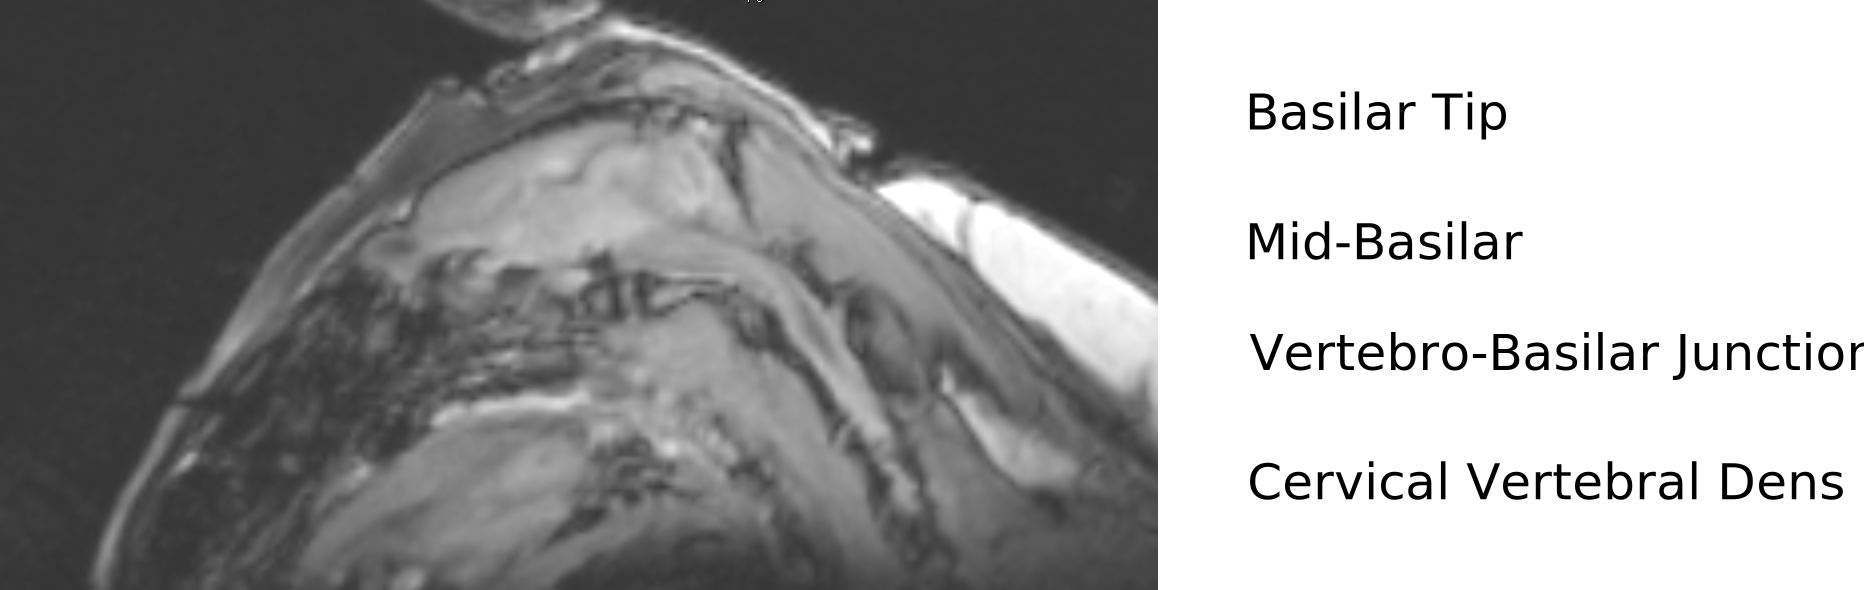
\includegraphics[scale=0.8]{brain.pdf}}
%\hspace{0.2cm}
%\raisebox{-0.5\height}{\includegraphics[scale=1.0]{../config/legend.pdf}} \\
%\vspace{0.5cm}
\begin{tabular}{m{5cm}m{20cm}}
SSVEP, 40.8333 Hz, Baseline Brain Recordings - no catheter in the rabbit - endo not hooked up &
\includegraphics[scale=0.150]{../ssvep/matlab_data/_Thu_24_04_2014_10_26_41_ssvep_.pdf} \\
12:03:18 - SSVEP 40 Hz, GND: Nose - Left Vert - angled glidecath @ osteum of left vert; recording from Ag/AgCl; GND: Nose &
\includegraphics[scale=0.150]{../ssvep/matlab_data/_Thu_24_04_2014_12_03_18_ssvep_.pdf} \\
12:59:49 - SSVEP 40 Hz, GND: Nose -X-pedion wire through echelon-10, basilar tip (via left vert); wire projects slightly beyond the catheter (documented on imaging) &
\includegraphics[scale=0.150]{../ssvep/matlab_data/_Thu_24_04_2014_12_59_49_ssvep_.pdf} \\
13:24:22 - SSVEP 40 Hz, GND: Nose -echelon-10, basilar tip (via left vert), Ag/AgCl electrode &
\includegraphics[scale=0.150]{../ssvep/matlab_data/_Thu_24_04_2014_13_24_22_ssvep_.pdf} \\
13:52:00 - SSVEP right eye 40 Hz, GND: Nose- X-pedion wire through echelon-10, wire is just at hub of catheter; catheter remains at basilar tip &
\includegraphics[scale=0.150]{../ssvep/matlab_data/_Thu_24_04_2014_13_52_00_ssvep_40hz.pdf} \\
14:08:34 - SSVEP, 42 Hz, GND: Nose- X-pedion wire, 100 cm (half-length), through echelon 10. Specifically: wire is 100 cm into the catheter (total length of wire is 200cm; hub of sidearm reaches 100cm from proximal end of wire) &
\includegraphics[scale=0.150]{../ssvep/matlab_data/_Thu_24_04_2014_14_08_34_ssvep_40.pdf} \\
%14:25:50 - SSVEP 40 Hz, GND: Nose -X-pedion wire, hub of sidearm reaches 47.3 cm from proximal end of wire (calculated so that wire is 10 cm from catheter tip (assuming 162.7 cm total catheter length: 150cm catheter shaft plus hub material that we measured by hand, plus the length of the sidearm) &
%14:52:20 - SSVEP, 40 Hz, GND: Nose - lights in room are OFF - X-pedion wire, repositioned just beyond tip of Echelon catheter at tip of basilar, confirmed with imaging; ALL ELECTRONICS ON, 4 PERSONNEL MOVING AND TALKING IN ROOM &
15:11:55 - SSVEP, 40 Hz - ELECTRONICS OFF (unchanged position X-pedion wire, repositioned just beyond tip of Echelon catheter at tip of basilar,) &
\includegraphics[scale=0.150]{../ssvep/matlab_data/_Thu_24_04_2014_15_11_55_ssvep_40.pdf} \\
15:51:40 - SSVEP, 40 Hz - Xpedion-10 still at basilar tip,  echelon-10 pulled back to C2 level (test intended to look at effect of having more exposed wire) &
\includegraphics[scale=0.150]{../ssvep/matlab_data/_Thu_24_04_2014_15_51_40_ssvep_40.pdf} \\
\end{tabular}
\caption{Rabbit 8 SSVEP 40 Hz.}
\end{center}
\end{figure}

\begin{figure}[H]
\begin{center}
%\raisebox{-0.5\height}{\includegraphics[scale=0.8]{brain.pdf}}
%\hspace{0.2cm}
%\raisebox{-0.5\height}{\includegraphics[scale=1.0]{../config/legend.pdf}} \\
%\vspace{0.5cm}
\begin{tabular}{m{5cm}m{20cm}}
16:14:30 - SSVEP, 40 Hz - Xpedion wire, just beyond echelon-10 catheter, both located at C2 level &
\includegraphics[scale=0.150]{../ssvep/matlab_data/_Thu_24_04_2014_16_14_30_ssvep_40.pdf} \\
16:38:01 - SSVEP, 40 Hz - Terumo 4Fr, Right cervical common carotid artery near C2 level, recording from Ag/AgCl &
\includegraphics[scale=0.150]{../ssvep/matlab_data/_Thu_24_04_2014_16_38_01_ssvep_40.pdf} \\
16:59:49 - SSVEP, 40Hz - DEAD ANIMAL CONTROLS - endo is Ag/AgCl Terumo 4 Fr, Right cervical common carotid artery near C2 level (same position as previous), recording from Ag/AgCl &
\includegraphics[scale=0.150]{../ssvep/matlab_data/_Thu_24_04_2014_16_59_49_ssvep_40.pdf}
\end{tabular}
\caption{Rabbit 8 SSVEP 40 Hz (continued).}
\end{center}
\end{figure}




\begin{figure}[H]
\begin{center}
%\raisebox{-0.5\height}{\includegraphics[scale=0.8]{brain.pdf}}
%\hspace{0.2cm}
%\raisebox{-0.5\height}{\includegraphics[scale=1.0]{../config/legend.pdf}} \\
%\vspace{0.5cm}
\begin{tabular}{m{5cm}m{20cm}}
SSVEP 51 Hz, X-pedion wire through echelon-10, basilar tip (via left vert); wire projects slightly beyond the catheter (documented on imaging) &
\includegraphics[scale=0.150]{../ssvep/matlab_data/_Thu_24_04_2014_13_01_58_ssvep_.pdf} \\
13:25:11 - SSVEP 51 Hz, GND: Nose -echelon-10, basilar tip (via left vert), Ag/AgCl electrode &
\includegraphics[scale=0.150]{../ssvep/matlab_data/_Thu_24_04_2014_13_25_11_ssvep_.pdf} \\
13:51:09 - SSVEP right eye 51 Hz, GND: Nose- X-pedion wire through echelon-10, wire is just at hub of catheter; catheter remains at basilar tip &
\includegraphics[scale=0.150]{../ssvep/matlab_data/_Thu_24_04_2014_13_51_09_ssvep_.pdf} \\
14:09:23 - SSVEP, 51 Hz, GND: Nose- X-pedion wire, 100 cm (half-length), through echelon 10. Specifically: wire is 100 cm into the catheter (total length of wire is 200cm; hub of sidearm reaches 100cm from proximal end of wire) &
\includegraphics[scale=0.150]{../ssvep/matlab_data/_Thu_24_04_2014_14_09_23_ssvep_.pdf} \\
14:24:53 - SSVEP, 50 Hz, GND: Nose -X-pedion wire, hub of sidearm reaches 47.3 cm from proximal end of wire (calculated so that wire is 10 cm from catheter tip (assuming 162.7 cm total catheter length: 150cm catheter shaft plus hub material that we measured by hand, plus the length of the sidearm) &
\includegraphics[scale=0.150]{../ssvep/matlab_data/_Thu_24_04_2014_14_24_53_ssvep_50.pdf} \\
%14:53:22 - SSVEP, 51 Hz, GND: Nose - lights in room are OFF - X-pedion wire, repositioned just beyond tip of Echelon catheter at tip of basilar, confirmed with imaging; ALL ELECTRONICS ON, 4 PERSONNEL MOVING AND TALKING IN ROOM &
15:11:00 - SSVEP, 51 Hz - ELECTRONICS OFF (unchanged position X-pedion wire, repositioned just beyond tip of Echelon catheter at tip of basilar,) &
\includegraphics[scale=0.150]{../ssvep/matlab_data/_Thu_24_04_2014_15_11_00_ssvep_50.pdf} \\
15:52:32 - SSVEP, 50 Hz - Xpedion-10 still at basilar tip,  echelon-10 pulled back to C2 level (test intended to look at effect of having more exposed wire) &
\includegraphics[scale=0.150]{../ssvep/matlab_data/_Thu_24_04_2014_15_52_32_ssvep_50.pdf} \\
\end{tabular}
\caption{Rabbit 8 SSVEP 50 Hz.}
\end{center}
\end{figure}

\begin{figure}[H]
\begin{center}
\begin{tabular}{m{5cm}m{20cm}}
16:13:39 - SSVEP, 50 Hz - Xpedion wire, just beyond echelon-10 catheter, both located at C2 level &
\includegraphics[scale=0.150]{../ssvep/matlab_data/_Thu_24_04_2014_16_13_39_ssvep_50.pdf} \\
16:15:20 - SSVEP, 10 Hz - Xpedion wire, just beyond echelon-10 catheter, both located at C2 level &
\includegraphics[scale=0.150]{../ssvep/matlab_data/_Thu_24_04_2014_16_15_20_ssvep_10.pdf} \\
16:37:09 - SSVEP, 10 Hz - Terumo 4Fr, Right cervical common carotid artery near C2 level, recording from Ag/AgCl &
\includegraphics[scale=0.150]{../ssvep/matlab_data/_Thu_24_04_2014_16_37_09_ssvep_10.pdf} \\
16:38:52 - SSVEP, 50 Hz - Terumo 4Fr, Right cervical common carotid artery near C2 level, recording from Ag/AgCl &
\includegraphics[scale=0.150]{../ssvep/matlab_data/_Thu_24_04_2014_16_38_52_ssvep_50.pdf} \\
16:58:54 - SSVEP, 50 Hz - DEAD ANIMAL CONTROLS - endo is Ag/AgCl Terumo 4 Fr, Right cervical common carotid artery near C2 level (same position as previous), recording from Ag/AgCl &
\includegraphics[scale=0.150]{../ssvep/matlab_data/_Thu_24_04_2014_16_58_54_ssvep_50.pdf} \\
17:00:39 - SSVEP, 10 Hz - DEAD ANIMAL CONTROLS - endo is Ag/AgCl Terumo 4 Fr, Right cervical common carotid artery near C2 level (same position as previous), recording from Ag/AgCl &
\includegraphics[scale=0.150]{../ssvep/matlab_data/_Thu_24_04_2014_17_00_39_ssvep_10.pdf} 
\end{tabular}
\caption{Rabbit 8 SSVEP 50 Hz (continued).}
\end{center}
\end{figure}

\end{document}
